\documentclass[]{book}
\usepackage{lmodern}
\usepackage{amssymb,amsmath}
\usepackage{ifxetex,ifluatex}
\usepackage{fixltx2e} % provides \textsubscript
\ifnum 0\ifxetex 1\fi\ifluatex 1\fi=0 % if pdftex
  \usepackage[T1]{fontenc}
  \usepackage[utf8]{inputenc}
\else % if luatex or xelatex
  \ifxetex
    \usepackage{mathspec}
  \else
    \usepackage{fontspec}
  \fi
  \defaultfontfeatures{Ligatures=TeX,Scale=MatchLowercase}
\fi
% use upquote if available, for straight quotes in verbatim environments
\IfFileExists{upquote.sty}{\usepackage{upquote}}{}
% use microtype if available
\IfFileExists{microtype.sty}{%
\usepackage{microtype}
\UseMicrotypeSet[protrusion]{basicmath} % disable protrusion for tt fonts
}{}
\usepackage[margin=1in]{geometry}
\usepackage{hyperref}
\hypersetup{unicode=true,
            pdftitle={Impacto programas PAES y PEAMA},
            pdfauthor={Daniel Rodriguez Chaves},
            pdfborder={0 0 0},
            breaklinks=true}
\urlstyle{same}  % don't use monospace font for urls
\usepackage{natbib}
\bibliographystyle{apalike}
\usepackage{color}
\usepackage{fancyvrb}
\newcommand{\VerbBar}{|}
\newcommand{\VERB}{\Verb[commandchars=\\\{\}]}
\DefineVerbatimEnvironment{Highlighting}{Verbatim}{commandchars=\\\{\}}
% Add ',fontsize=\small' for more characters per line
\usepackage{framed}
\definecolor{shadecolor}{RGB}{248,248,248}
\newenvironment{Shaded}{\begin{snugshade}}{\end{snugshade}}
\newcommand{\KeywordTok}[1]{\textcolor[rgb]{0.13,0.29,0.53}{\textbf{#1}}}
\newcommand{\DataTypeTok}[1]{\textcolor[rgb]{0.13,0.29,0.53}{#1}}
\newcommand{\DecValTok}[1]{\textcolor[rgb]{0.00,0.00,0.81}{#1}}
\newcommand{\BaseNTok}[1]{\textcolor[rgb]{0.00,0.00,0.81}{#1}}
\newcommand{\FloatTok}[1]{\textcolor[rgb]{0.00,0.00,0.81}{#1}}
\newcommand{\ConstantTok}[1]{\textcolor[rgb]{0.00,0.00,0.00}{#1}}
\newcommand{\CharTok}[1]{\textcolor[rgb]{0.31,0.60,0.02}{#1}}
\newcommand{\SpecialCharTok}[1]{\textcolor[rgb]{0.00,0.00,0.00}{#1}}
\newcommand{\StringTok}[1]{\textcolor[rgb]{0.31,0.60,0.02}{#1}}
\newcommand{\VerbatimStringTok}[1]{\textcolor[rgb]{0.31,0.60,0.02}{#1}}
\newcommand{\SpecialStringTok}[1]{\textcolor[rgb]{0.31,0.60,0.02}{#1}}
\newcommand{\ImportTok}[1]{#1}
\newcommand{\CommentTok}[1]{\textcolor[rgb]{0.56,0.35,0.01}{\textit{#1}}}
\newcommand{\DocumentationTok}[1]{\textcolor[rgb]{0.56,0.35,0.01}{\textbf{\textit{#1}}}}
\newcommand{\AnnotationTok}[1]{\textcolor[rgb]{0.56,0.35,0.01}{\textbf{\textit{#1}}}}
\newcommand{\CommentVarTok}[1]{\textcolor[rgb]{0.56,0.35,0.01}{\textbf{\textit{#1}}}}
\newcommand{\OtherTok}[1]{\textcolor[rgb]{0.56,0.35,0.01}{#1}}
\newcommand{\FunctionTok}[1]{\textcolor[rgb]{0.00,0.00,0.00}{#1}}
\newcommand{\VariableTok}[1]{\textcolor[rgb]{0.00,0.00,0.00}{#1}}
\newcommand{\ControlFlowTok}[1]{\textcolor[rgb]{0.13,0.29,0.53}{\textbf{#1}}}
\newcommand{\OperatorTok}[1]{\textcolor[rgb]{0.81,0.36,0.00}{\textbf{#1}}}
\newcommand{\BuiltInTok}[1]{#1}
\newcommand{\ExtensionTok}[1]{#1}
\newcommand{\PreprocessorTok}[1]{\textcolor[rgb]{0.56,0.35,0.01}{\textit{#1}}}
\newcommand{\AttributeTok}[1]{\textcolor[rgb]{0.77,0.63,0.00}{#1}}
\newcommand{\RegionMarkerTok}[1]{#1}
\newcommand{\InformationTok}[1]{\textcolor[rgb]{0.56,0.35,0.01}{\textbf{\textit{#1}}}}
\newcommand{\WarningTok}[1]{\textcolor[rgb]{0.56,0.35,0.01}{\textbf{\textit{#1}}}}
\newcommand{\AlertTok}[1]{\textcolor[rgb]{0.94,0.16,0.16}{#1}}
\newcommand{\ErrorTok}[1]{\textcolor[rgb]{0.64,0.00,0.00}{\textbf{#1}}}
\newcommand{\NormalTok}[1]{#1}
\usepackage{longtable,booktabs}
\usepackage{graphicx,grffile}
\makeatletter
\def\maxwidth{\ifdim\Gin@nat@width>\linewidth\linewidth\else\Gin@nat@width\fi}
\def\maxheight{\ifdim\Gin@nat@height>\textheight\textheight\else\Gin@nat@height\fi}
\makeatother
% Scale images if necessary, so that they will not overflow the page
% margins by default, and it is still possible to overwrite the defaults
% using explicit options in \includegraphics[width, height, ...]{}
\setkeys{Gin}{width=\maxwidth,height=\maxheight,keepaspectratio}
\IfFileExists{parskip.sty}{%
\usepackage{parskip}
}{% else
\setlength{\parindent}{0pt}
\setlength{\parskip}{6pt plus 2pt minus 1pt}
}
\setlength{\emergencystretch}{3em}  % prevent overfull lines
\providecommand{\tightlist}{%
  \setlength{\itemsep}{0pt}\setlength{\parskip}{0pt}}
\setcounter{secnumdepth}{5}
% Redefines (sub)paragraphs to behave more like sections
\ifx\paragraph\undefined\else
\let\oldparagraph\paragraph
\renewcommand{\paragraph}[1]{\oldparagraph{#1}\mbox{}}
\fi
\ifx\subparagraph\undefined\else
\let\oldsubparagraph\subparagraph
\renewcommand{\subparagraph}[1]{\oldsubparagraph{#1}\mbox{}}
\fi

%%% Use protect on footnotes to avoid problems with footnotes in titles
\let\rmarkdownfootnote\footnote%
\def\footnote{\protect\rmarkdownfootnote}

%%% Change title format to be more compact
\usepackage{titling}

% Create subtitle command for use in maketitle
\newcommand{\subtitle}[1]{
  \posttitle{
    \begin{center}\large#1\end{center}
    }
}

\setlength{\droptitle}{-2em}
  \title{Impacto programas PAES y PEAMA}
  \pretitle{\vspace{\droptitle}\centering\huge}
  \posttitle{\par}
  \author{Daniel Rodriguez Chaves}
  \preauthor{\centering\large\emph}
  \postauthor{\par}
  \predate{\centering\large\emph}
  \postdate{\par}
  \date{2018-05-16}

\usepackage{booktabs}

\usepackage{amsthm}
\newtheorem{theorem}{Teorema}[chapter]
\newtheorem{lemma}{Lema}[chapter]
\theoremstyle{definition}
\newtheorem{definition}{Definición}[chapter]
\newtheorem{corollary}{Corolario}[chapter]
\newtheorem{proposition}{Proposición}[chapter]
\theoremstyle{definition}
\newtheorem{example}{Ejemplo}[chapter]
\theoremstyle{definition}
\newtheorem{exercise}{Ejercicio}[chapter]
\theoremstyle{remark}
\newtheorem*{remark}{Remarcación }
\newtheorem*{solution}{Solución}
\begin{document}
\maketitle

{
\setcounter{tocdepth}{1}
\tableofcontents
}
\chapter{Introducción}\label{introduccion}

Con el objetivo de analizar el impacto que han tenido los programas PAES
y PEAMA con respecto a la admisión a la Universidad Nacional de Colombia
de las poblaciones menos favorecidas de tal manera que exista equidad,
además de medir el impacto de los programas de bienestar universitario
sobre la permanencia y culminación de los procesos académicos de los
estudiantes pertenecientes a los programas PAES y PEAMA se propusieron
metodologías estadísticas que permiten llevar a cabo tales mediciones
que se propuso como tarea en la Dirección Nacional de Bienestar
Universitario.

\emph{sample} \textbf{Markdown} \url{https://yihui.name/tinytex/}.

\chapter{Objetivos}\label{obj}

\section{OBJETIVO GENERAL}\label{objetivo-general}

Llevar a cabo a través de técnicas estadísticas un estudio del impacto
de los programas de admisión especial (PAES y PEAMA) en términos de
admisión, permanencia y graduación, en el marco de las políticas de
inclusión educativa en la Universidad Nacional de Colombia

\section{OBJETIVOS ESPECIFICOS}\label{objetivos-especificos}

\begin{itemize}
\tightlist
\item
  Presentar una descripción del panorama general de los estudiantes de
  nuestra población de estudio con respecto a la admisión, permanecía y
  graduación.
\item
  Validar las normas aplicadas al momento de admisión para los programas
  PAES y PEAMA.
\item
  Llevar a cabo la medición del impacto de los programas PAES y PEAMA a
  los estudiantes en el momento de la admisión.
\item
  Llevar a cabo la medición del impacto de los programas que Bienestar
  ofrece a los estudiantes PAES y PEAMA durante su permanencia en las
  áreas de acompañamiento integral, gestión y fomento socioeconómico,
  salud, cultura y deportes.
\end{itemize}

\section{Ignorar por ahora}\label{ignorar-por-ahora}

You can label chapter and section titles using \texttt{\{\#label\}}
after them, e.g., we can reference Chapter \ref{obj}. If you do not
manually label them, there will be automatic labels anyway, e.g.,
Chapter \ref{methods}.

Figures and tables with captions will be placed in \texttt{figure} and
\texttt{table} environments, respectively.

\begin{Shaded}
\begin{Highlighting}[]
\KeywordTok{par}\NormalTok{(}\DataTypeTok{mar =} \KeywordTok{c}\NormalTok{(}\DecValTok{4}\NormalTok{, }\DecValTok{4}\NormalTok{, .}\DecValTok{1}\NormalTok{, .}\DecValTok{1}\NormalTok{))}
\KeywordTok{plot}\NormalTok{(pressure, }\DataTypeTok{type =} \StringTok{'b'}\NormalTok{, }\DataTypeTok{pch =} \DecValTok{19}\NormalTok{)}
\end{Highlighting}
\end{Shaded}

\begin{figure}

{\centering 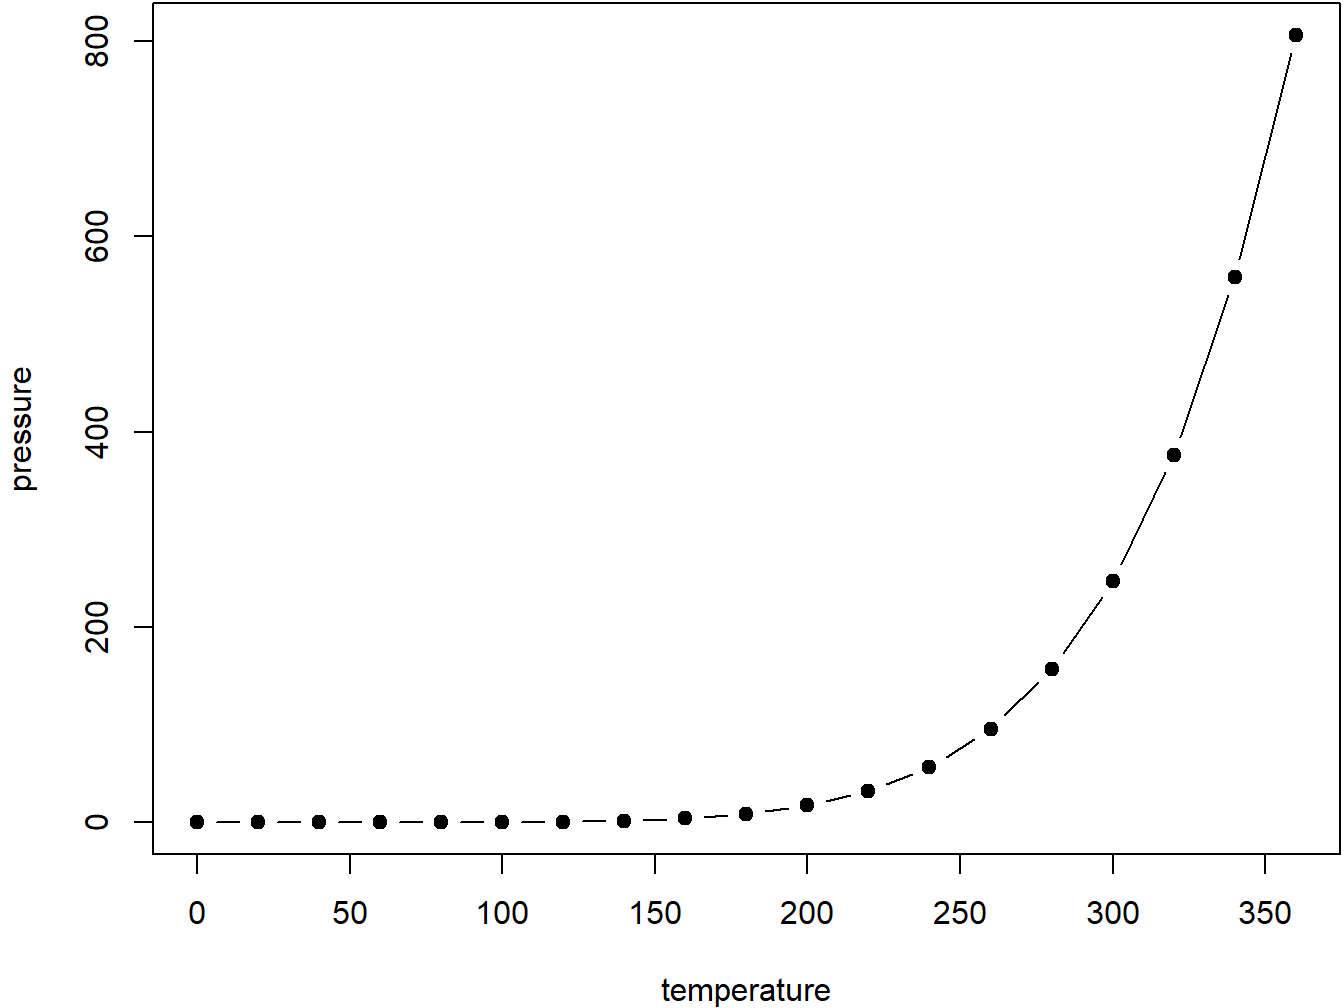
\includegraphics[width=0.8\linewidth]{bookdown_files/figure-latex/nice-fig-1} 

}

\caption{Here is a nice figure!}\label{fig:nice-fig}
\end{figure}

Reference a figure by its code chunk label with the \texttt{fig:}
prefix, e.g., see Figure \ref{fig:nice-fig}. Similarly, you can
reference tables generated from \texttt{knitr::kable()}, e.g., see Table
\ref{tab:nice-tab}.

\begin{Shaded}
\begin{Highlighting}[]
\NormalTok{knitr}\OperatorTok{::}\KeywordTok{kable}\NormalTok{(}
  \KeywordTok{head}\NormalTok{(iris, }\DecValTok{3}\NormalTok{), }\DataTypeTok{caption =} \StringTok{'Here is a nice table!'}\NormalTok{,}
  \DataTypeTok{booktabs =} \OtherTok{TRUE}
\NormalTok{)}
\end{Highlighting}
\end{Shaded}

\begin{table}

\caption{\label{tab:nice-tab}Here is a nice table!}
\centering
\begin{tabular}[t]{rrrrl}
\toprule
Sepal.Length & Sepal.Width & Petal.Length & Petal.Width & Species\\
\midrule
5.1 & 3.5 & 1.4 & 0.2 & setosa\\
4.9 & 3.0 & 1.4 & 0.2 & setosa\\
4.7 & 3.2 & 1.3 & 0.2 & setosa\\
\bottomrule
\end{tabular}
\end{table}

You can write citations, too. For example, we are using the
\textbf{bookdown} package \citep{R-bookdown} in this sample book, which
was built on top of R Markdown and \textbf{knitr} \citep{xie2015}.

\mainmatter

\chapter{MARCO CONCEPTUAL}\label{marco}

\section{Análisis de correspondencias
múltiples}\label{analisis-de-correspondencias-multiples}

Como se presenta en Pardo \citep[pp.~125 - 163]{Pardo}, el análisis de
correspondencias múltiples es una herramienta estadística cuyo objetivo
es analizar asociaciones entre categorías de las variables de interés,
esto a través de métodos gráficos que permitan observar cuales
categorías de una variable son las que más afectan a las diferentes
categorías de las otras variables, además permite reducir la dimensión
de la matriz de datos de tal manera que se pueda llegar a observar las
relaciones de las categorías usando un gráfico bidimensional. Se puede
entender como un análisis de correspondencias simples aplicado a una
tabla disyuntiva completa o bien aplicado a la tabla de Burt
correspondiente teniendo en cuenta que en este caso se pierde la
información por individuo. El método, como ya se dijo, se puede entender
como la generalización de un análisis de correspondencias simple al caso
de más de dos variables categóricas de interés, pero también se puede
entender como la realización de dos diferentes análisis de componentes
principales, uno de ellos permite hacer los cálculos de una manera
relativamente sencilla y el otro ayuda a llevar a cabo la interpretación
de los ejes obtenidos, en general, esta interpretación se hace
únicamente sobre las categorías de las variables y no sobre los
individuos ya que los últimos son, en la mayoría de los casos, anónimos.
Para seleccionar el número de ejes a retener se usan dos metodologías,
la primera es elegir el número a través del histograma de valores
propios de los ejes de acuerdo a la cantidad de valores propios que se
puedan considerar diferentes, y si hay muchos valores propios similares
se considera que pertenecen a ejes ``parásitos'', es decir a ejes que no
brindan más información. La segunda metodología se conoce como el
criterio de Benzecri, dentro de los ejes cuyo valor propio sea mayor al
inverso del número de categorías dentro del análisis se recalcula las
tasas de inercia y se selecciona el número de ejes a través del
histograma de las tasas de inercia recalculadas de la misma manera que
se hizo con el histograma de valores propios. El análisis de
correspondencias múltiples permite, además, incluir la proyección de
variables que no participaron en la construcción de los ejes, a estas
variables se les conoce como suplementarias y sirve para describir las
posibles relaciones que presentan esas categorías suplementarias con las
categorías de las variables activas del análisis.

\section{Modelos multinomiales}\label{modelos-multinomiales}

Cuando en un problema de modelación estadística, la variable dependiente
o de respuesta es de tipo categórico nominal una de las opciones para
llevar a cabo el análisis es recurrir a modelos logit de categoría base
adecuados a respuestas de tipo nominal \citep[pp.~267]{Agresti}. Este
modelo, también conocido como modelo multinomial, es un análisis
conjunto de modelos logit binarios para cada par de categorías como se
observa en la ecuación (1):

\[\log { \left( \frac { { \pi  }_{ j } }{ { \pi  }_{ J } }  \right)  } ={ \alpha  }_{ j }+{ \beta  }_{ j }x,\quad \quad \quad j=1,\cdots ,J-1 \quad \quad(1)\]

Donde \(J\) es el número total de categórias, \(x\) es una matriz cuyas
columnas corresponden a las variables explicativas, \({ \alpha }_{ j }\)
y \({ \beta }_{ j }\) son los parámetros a estimar en el modelo y
\({ \pi }_{ j }(x)=P(Y=j|x)\) las probabilidades asociadas a cada una de
las categorías de la variable respuesta \(Y\) con
\(\sum _{ j=1 }^{ J }{ { \pi }_{ j }(x) } =1\). Nótese que se puede
hallar la asociación de cualquier par de categorías a través de la
ecuación (2):

\[\log { \left( \frac { { \pi  }_{ a } }{ { \pi  }_{ b } }  \right)  } =\log { \left( \frac { { \pi  }_{ a } }{ { \pi  }_{ J } }  \right)  } -\log { \left( \frac { { \pi  }_{ b } }{ { \pi  }_{ J } }  \right)  } \quad \quad (2)\]

Para llevar a cabo la comparación entre modelos y poder seleccionar el
más adecuado, en términos de cuáles son las variables que lo van a
conformar y de la parsimonia del modelo, se usa el AIC o criterio de
información de Akaike, el cual evalúa al modelo de acuerdo a la cercanía
entre los valores ajustados a través del modelo y los verdaderos valores
penalizando por el número de parámetros \citep[pp.~216]{Agresti} y
permite comparar el ajuste de modelos que no están anidados. Cuando se
usa el AIC el modelo que más se ajusta a los datos será aquel que tenga
menor AIC y también se usa el BIC o criterio de información bayesiano,
el cual es muy similar al AIC, pero además toma en cuenta el tamaño de
la muestra \citep[pp.~257]{Agresti}. El proceso que se lleva a cabo para
la selección del modelo se conoce como backward o eliminación hacia
atrás, y se conduce como en \citet[ pp.~214]{Agresti}, es decir se parte
del modelo más completo y se elimina un parámetro a la vez. Para llevar
a cabo la estimación de las probabilidades de respuesta a través del
modelo se aplica la fórmula (3):

\[{ \hat { \pi  }  }_{ j }(x)=\frac { exp({ \hat { \alpha  }  }_{ j }+{ \hat { \beta ' }  }_{ j }x) }{ 1+\sum _{ h=1 }^{ J-1 }{ exp({ \hat { \alpha  }  }_{ h }+{ \hat { \beta ' }  }_{ h }x) }  } \quad \quad (3)\]

Y como se observa en la ecuación (4), los parámetros se pueden
interpretar a través del logit de una probabilidad condicional:

\[\log { \left( \frac { { \pi  }_{ j } }{ { \pi  }_{ J } }  \right)  } =\log { \left( \frac { \left( \frac { { \pi  }_{ j } }{ { \pi  }_{ J }+{ \pi  }_{ j } }  \right)  }{ \left( \frac { { \pi  }_{ J } }{ { \pi  }_{ J }+{ \pi  }_{ j } }  \right)  }  \right)  } =\log { \left( \frac { \left( \frac { { \pi  }_{ j } }{ { \pi  }_{ J }+{ \pi  }_{ j } }  \right)  }{ 1-\left( \frac { { \pi  }_{ j } }{ { \pi  }_{ J }+{ \pi  }_{ j } }  \right)  }  \right)  } =logit\left( \frac { { \pi  }_{ j } }{ { \pi  }_{ J }+{ \pi  }_{ j } }  \right) \quad \quad (4)\]

\section{Modelos multinomiales logísticos
multinivel}\label{modelos-multinomiales-logisticos-multinivel}

Los modelos multinivel aparecen, principalmente, en aplicaciones de la
estadística para hacer análisis con respecto a la educación
\citep{Goldstein}. Surgen como una ampliación a los modelos
generalizados ya existentes, para los cuales uno de sus supuestos
básicos es la independencia de las observaciones, pero al observar que
los individuos que se están analizando se encuentran agrupados
(estudiantes dentro de salones, salones dentro de colegios, etc\ldots{})
y que dentro de los grupos los individuos, en general, son similares
pero entre grupos existen diferencias más claras, es decir, se viola el
supuesto de independencia los modelos existentes ya no son válidos en
este caso. En términos simples, el modelo multinivel hace una corrección
al problema de independencia a través de la inclusión de variables
aleatorias correspondientes a los múltiples niveles de anidación de
nuestros datos y que permiten llevar cabo estimaciones correctas de los
parámetros del modelo. Para nuestro caso el modelo de interés es de
respuesta categórica nominal, de ahí que el modelo a usar resulte un
modelo multinomial logístico multinivel \citep{Goldstein} de manera en
que se especifica en la fórmula (5):

\[\log { \left( \frac { { { \pi  }_{ j } }^{ (s) } }{ { { \pi  }_{ J } }^{ (s) } }  \right)  } ={ \alpha  }_{ j }+{ \beta  }_{ j }{ x }^{ (s) }+{ { u }_{ j } }^{ (s) },\quad \quad \quad j=1,\cdots ,J-1\quad \quad (5)\]

Donde \(J\) es el número total de categórias, x es una matriz cuyas
columnas corresponden a las variables explicativas, \({ \alpha }_{ j }\)
y \({ \beta }_{ j }\) son los parámetros a estimar en el modelo, \(s\)
es el nivel de agrupación de las observaciones y
\({ { \pi }_{ j } }^{ (s) }({ x }^{ (s) })=P(Y=j|{ x }^{ (s) },s)\) las
probabilidades asociadas a cada una de las categorías de la variable
respuesta Y en cada uno de los niveles (\(S\)),
\(\sum _{ j=1 }^{ J }{ \sum _{ s=1 }^{ S }{ { { \pi }_{ j } }^{ (s) }(x) } } =1\)
y el \({ { u }_{ j } }^{ (s) }\) es un error aleatorio asociado a cada
nivel. Se tienen como opciones la cuasi verosimilitud, la máxima
verosimilitud o los procedimientos MCMC para la estimación de los
parámetros. Pero como se presenta en \citep{HadfieldBook}:

\emph{``En el contexto de los modelos lineales generalizados mixtos
(GLMM), aquí está lo que yo observo como los pros y los contras de usar
máxima verosimilitud (restringida - REML) versus los métodos bayesianos
de Cadenas de Markov de Monte Carlo (MCMC). REML son rápidos y fáciles
de usar, mientras los métodos MCMC pueden ser lentos y más retadores
técnicamente. En particular, el reto es la especificación de una apiori
sensible, el cual no es una dificultad con REML. Sin embargo, los
resultados analíticos para GLMM no Gaussianos en general no están
disponibles y REML se basa en procedimientos que usan métodos de máxima
verosimilitud aproximada que pueden no funcionar bien. MCMC también es
una aproximación, pero la exactitud de la aproximación incrementa en la
misma medida que aumenta la longitud del análisis, siendo exactos al
límite. Adicionalmente REML usa teoría de grandes muestras para derivar
las aproximaciones de los intervalos de confianza los cuales pueden ser
muy pobres especialmente para las varianzas. Nuevamente, las medidas de
confianza de MCMC son exactas, excepto por el error de Monte Carlo, y
proveen de una manera fácil e intuitiva de obtener medidas de confianza
derivadas de las estadísticas como las razones de varianza,
correlaciones y predicciones.''}

Luego para tamaños de muestra grandes y siempre que los métodos
computacionales estén disponibles se puede acudir a métodos de
estimación REML, en los demás casos la solución será acudir a métodos de
estimación MCMC. Para más detalles sobre la estimación de parámetros de
los modelos multinivel desde la perspectiva frecuentista de los modelos
multinivel véase (Goldstein, 2010) y para la estimación de los
parámetros desde la perspectiva bayesiana véase \citep{Goldstein} y/o
\citep{HadfieldBook}. Para validar los supuestos y ajuste de los modelos
multinivel existen dos caminos a seguir y dependen de la manera en que
decidamos hacer la estimación de los parámetros de nuestro modelo. En la
primera manera, es decir, la frecuentista o REML los supuestos son: en
primera medida que los datos provengan de la distribución de
probabilidades teorizada por el modelo, pero a diferencia de los modelos
lineales generalizados usuales, los modelos multinivel no requieren la
independencia de los errores. En la segunda manera, es decir, la
bayesiana o MCMC los supuestos son: que los datos provengan de la
distribución de probabilidades teorizada por el modelo, que la
distribución a priori (que puede, o no, ser informativa) conjugue con la
función de máxima verosimilitud de los datos, además se debe verificar
que las cadenas de Márkov converjan para la estimación de los
parámetros. Al llevar a cabo las verificaciones anteriormente descritas
y apropiadas al método usado para la estimación entonces se garantiza
que nuestro modelo ha sido validado y que el mismo se ha ajustado a
nuestros datos.

\section{Software estadístico R:}\label{software-estadistico-r}

R es un leguaje y ambiente de computación estadístico de código libre
(GNU project) construido para dar sentido y valor agregado a los datos.
R provee de una muy amplia variedad de herramientas estadísticas la cual
es alimentada por su activa y creciente comunidad de colaboradores y
usuarios. RStudio es una IDE (entorno de desarrollo integrado) para R,
la comunidad de desarrolladores de RStudio inspirados por las
innovaciones de los usuarios de R en las ciencias, educación e industria
desarrollaron gran cantidad de herramientas, la mayoría libres, que
permite dar gran valor añadido a los datos (dashboards, htmlwidgets,
libros, etc\ldots{}) y para que los equipos de trabajo puedan promover y
compartir el trabajo posicionando a R como el lenguaje estadístico, de
inteligencia de negocios y de ciencia de datos más poderoso, innovador y
de mayor crecimiento en el mundo. Entre la gran variedad de librerías
que posee R describiremos a continuación aquellas que fueron utilizadas
en el desarrollo del proyecto. \textbf{Referencias:} \citep{r1},
\citep{wikiR}, \citep{wikiRStudio}, \citep{rstudio1}, \citep{rstudio2}.

\subsection{Librería tidyverse:}\label{libreria-tidyverse}

Es una colección de paquetes de R diseñados para ciencia de datos. Todos
los paquetes comparten una filosofía de diseño subyacente, gramática y
estructuras de datos. Contiene ggplot2 la cual es una librería poderosa
para hacer gráficos estáticos por capas, dplyr la cual sirve para la
manipulación de datos, tidyr la cual ayuda a depurar las bases de datos,
readr para la lectura de datos rectangulares, readxl para la lectura de
archivos .xls y .xlsx, purrr la cual permite hacer programación
funcional, tibble la cual es una manera moderna de pensar las
estructuras de datos, stringr la cual se encarga de que el trabajo con
caracteres (strings) sea lo más sencillo posible, forcats la cual
permite solucionar problemas frecuentes con la manipulación de factores,
entre otros muchos paquetes. \textbf{Referencias:} \citep{tidyverse}

\subsection{Librería Factoclass:}\label{libreria-factoclass}

Como lo describe dos de sus autores Campo Elías Pardo (profesor asociado
del Departamento de Estadística de la Universidad Nacional de Colombia)
y Pedro César del Campo (Estadístico de la Universidad Nacional de
Colombia) en \citep{Pardo2007}, el paquete se implementó con la
finalidad de llevar a cabo exploración multivariada de datos de acuerdo
con las estrategias descritas en \citep{Lebart} . \textbf{Referencias:}
\citep{Factoclass}

\subsection{Librería lme4:}\label{libreria-lme4}

Es una librería construida para el ajuste de modelos lineales de efectos
mixtos y modelos lineales generalizados de efectos mixtos desde un
enfoque de máxima verosimilitud restringida. \textbf{Referencias:}
\citep{lme4}, \citep{Bates}

\subsection{Librería MCMCglmm:}\label{libreria-mcmcglmm}

Es una librería de R la cual tiene como objetivo ajustar modelos
lineales generalizados mixtos con un enfoque bayesiano a través del uso
de Cadenas de Markov Monte Carlo (MCMC). \textbf{Referencias:}
\citep{MCMCglmm}, \citep{HadfieldBook}, \citep{HadfieldCourseNotes}.

\chapter{Metodología}\label{metodologuxeda}

La metodología llevada a cabo se divide en hacer análisis para los
estudiantes PAES y para los estudiantes PEAMA, que ingresaron en la
cohorte 2011-01, por separado. La metodología en ambos casos es la misma
y consta de los siguientes pasos:

\begin{enumerate}
\def\labelenumi{\arabic{enumi}.}
\tightlist
\item
  Construcción descriptiva del panorama de admisión de cada una de las
  dos poblaciones (PEAMA y PAES).
\item
  Revisión de la normatividad existente al ingreso de los dos grupos y
  su posterior validación.
\item
  Construcción de un único modelo binomial logit multinivel global de
  admisión.
\item
  Construcción de análisis de correspondencias múltiples para las
  variables incluidas en la permanencia y graduación que permita
  comprender cuales van a ser incluidas en el modelo para cada uno de
  los dos grupos de estudiantes (PAES y PEAMA).
\item
  Construcción de dos modelos multinomiales logit multinivel para cada
  uno de los grupos estudiantiles (PAES y PEAMA) que permita analizar
  permanencia y egreso de los estudiantes.
\end{enumerate}

\chapter{Admisión PAES}\label{admision-paes}

En este capítulo se presenta una descripción del panorama general de
admisión de los estudiantes PAES de la cohorte 2011-01.

\chapter{Admisión PEAMA}\label{admision-peama}

En este capítulo se presenta una descripción del panorama general de
admisión de los estudiantes PEAMA de la cohorte 2011-01.

\bibliography{book.bib,packages.bib}


\end{document}
